\chapter{Other malware}

In this chapter we will analyze other IoT malware that have been discovered in the last years. We will focus on the following malware: Hajime, Goldoon, and BotenaGo. In \Cref{fig:malware-architectures} going from centralized ones, in which there is a single CNC that controls the botnet to the P2P ones, in which the bots communicate with each other and lastly the hybrid ones, which are a mix of the two.

In centralized botnets, the bots sends out periodic signals to notify the CNC server of their presence. The CNC can directly issue commands to the bots, however, it also serves as a \textbf{single point of failure}: if it is taken down, the entire botnet becomes inoperative. In P2P botnets, the bots function as both CNC and clients that receive commands. This design eliminates the single point of failure, and for this reason they are more difficult to shut down. 

\begin{figure}[ht]
	\centering
	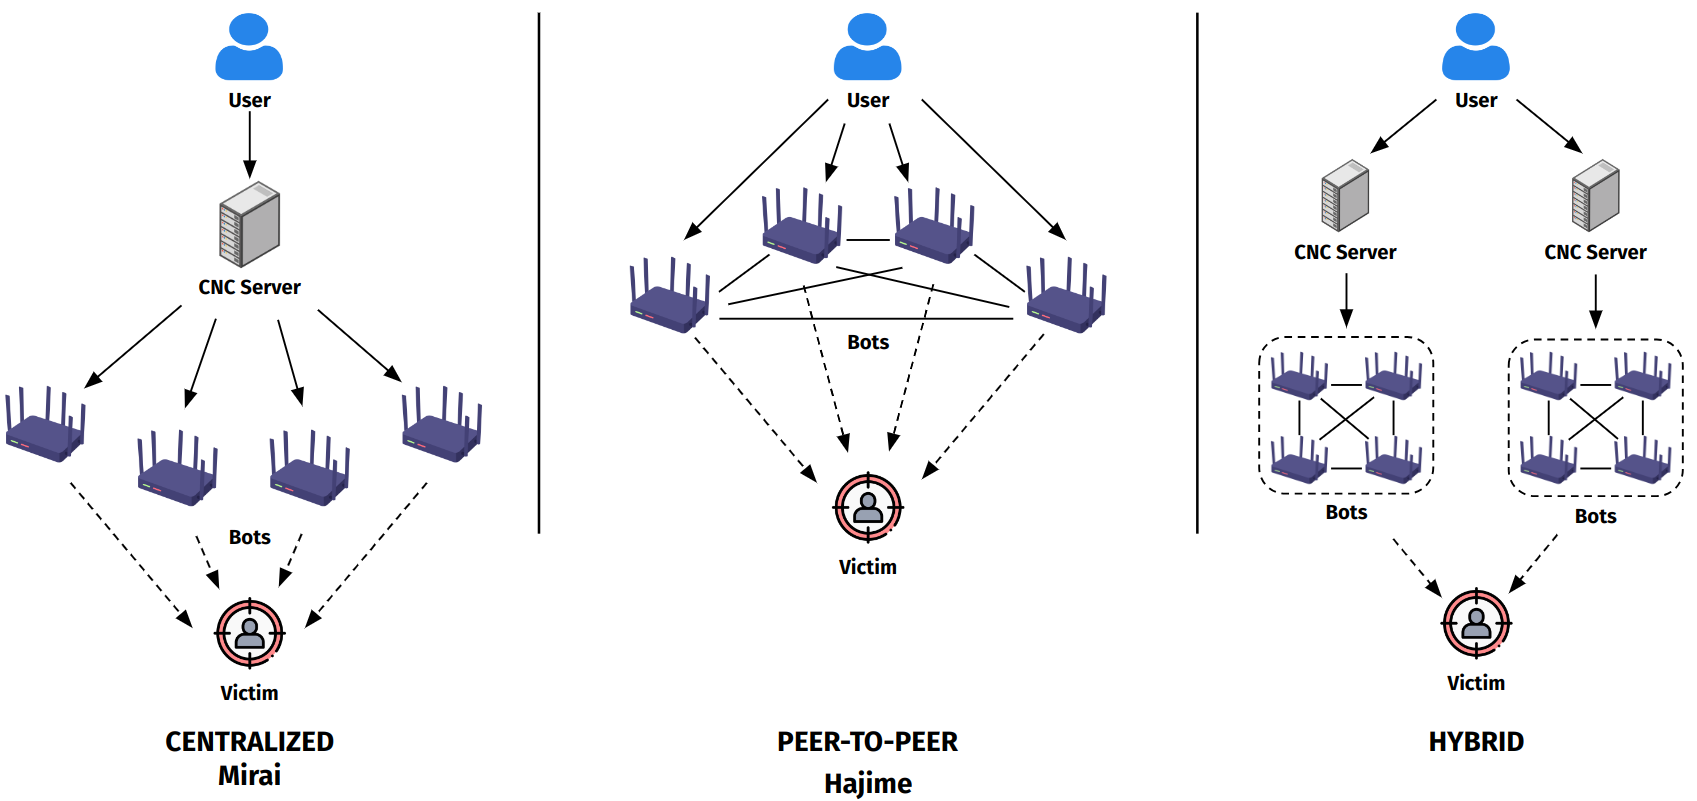
\includegraphics[scale=0.25]{resources/images/malware-architectures.png}
	\caption{Malware architectures}
	\label{fig:malware-architectures}
\end{figure}

\section{Hajime}

Hajime was first discovered in October 2016 by security researchers at Rapidity Networks, and it was given a Japanese name (meaning "beginning") thanks to its closed resemblance to Mirai. It mainly targets and infects IoT devices, exploiting default credentials and unpatched vulnerabilities. Once a device is infected, Hajime propagates itself by scanning the network and brute forcing credentials to gain access to the other devices. Unlike Mirai, Hajime has a decentralized P2P architecture, using a modified version of the BitTorrent protocol for communication. Another important difference is that, as of now, Hajime does not deliver any malicious payload, and it seems that it secures the devices it infects, specifically, it blocks ports 23, 7547, 5555, and 5358, which are commonly used by other malware to infect devices, effectively preventing infection from others. There are different speculations related to the motivations behind Hajime, some say that it could be a vigilante malware, designed to protect IoT devices, or it could be a future threat.

\section{Goldoon}
Goldoon is a malware which had a peak in terms of infected devices in April 2024 which is the same period in which researchers from Fortinet found about this new botnet~\cite{fortinet-goldoon}. The first difference between Goldoon and Mirai is in the targets and how it infects devices. Mirai targets IoT devices and tries to connect to them using default credentials, on the other hand Goldoon targets specifically D-Link DIR-645 which are vulnerable to the CVE-2015-2051~\cite{CVE-2015-2051}. This vulnerability allows for remote code execution on affected devices allowing the attackers to load Goldoon on the routers. In the same way as Mirai, Goldoon removes all the traces of its presence by removing the installation file. Moreover, Goldoon also goes through some system files to remove its traces. Another difference between the two is that Goldoon is persistent and can start in three different steps depending on the necessity:
\begin{enumerate}
    \item Boot: by inserting a cron job in the system or editing \texttt{init.d} folder files.
    \item Daemon: adding itself as a service.
    \item Logon: adding an entry in the \texttt{~/.bashrc} file or in \texttt{~/.config/autostart} of the Desktop.
\end{enumerate}
In terms of attack Goldoon provides a suite which is similar to the one offered by Mirai.

\section{BotenaGo}

Identified in November 2021 by AT\&T Alien Labs researchers, BotenaGo is a backdoor that provides cybercriminals access to devices through 33 exploit functions. Their first analysis was performed by reverse engineering the malware's binary, and it revealed that the malware associates each exploit function with a string that represents a potential target system, similar to a signature. This is needed because the malware sends a ``GET'' request to the target and then searches into the returned data for the signature. For example the string ``\texttt{Server: Boa/0.93.15}'' is mapped to the function \texttt{main\_infectFunctionGponFiber} which exploit the CVE-2020-8958 vulnerability. They also provide a search result on Shodan that shows 2 million potential targets. This number decreased in the years as you can see in \Cref{fig:boa-shodan}. All the exploits can be found in \Cref{fig:all-vulnerabilities-botenago} which illustrates the \texttt{scannerInitExploit} from its source code.

\begin{figure}[ht]
    \centering
    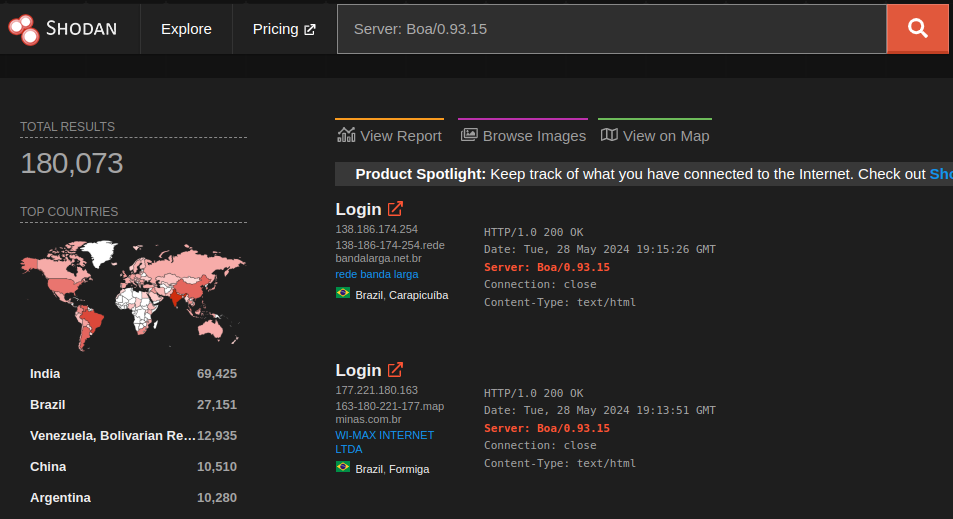
\includegraphics[scale=0.4]{resources/images/boa-shodan.png}
    \caption{Shodan search result for Boa/0.93.15}
    \label{fig:boa-shodan}
\end{figure}

The CNC has two ways of sending command to the infected device:

\begin{enumerate}
    \item Use one of the two backdoor ports (31412 and 19412) to send a command to the device. On port 19412, it listens for the victim IP address and once received it tries each exploit on that IP.
    \item It listens on a system IO user input. For example, it can be accessed locally by using telnet. 
\end{enumerate}

In 2022 its source code was leaked on GitHub and AT\&T Alien Labs provided another analysis which did not provide new information but confirmed the previous analysis. \cite{att-botenago-reverse,att-botenago-sourcecode}

\begin{figure}[ht]
    \centering
    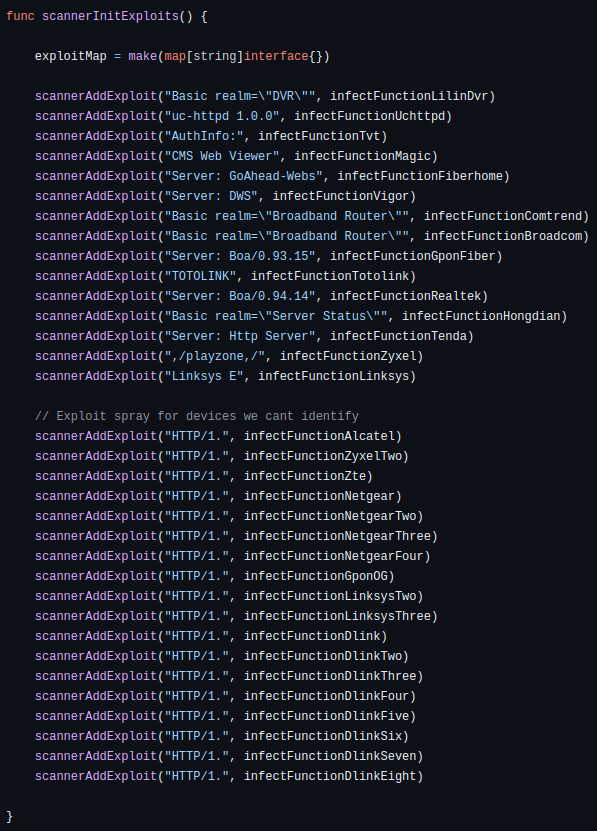
\includegraphics[scale=0.5]{resources/images/all-vulnerabilities-botenago.png}
    \caption{All the vulnerabilities exploited by BotenaGo}
    \label{fig:all-vulnerabilities-botenago}
\end{figure}

\paragraph{Comparison.} In table \ref{tab:malware_characteristics} we can see a summary of the comparison between the different malware.

\begin{table}[ht]
	\centering
	\begin{tabular}{|c|c|c|c|c|}
		\hline
		 & \textbf{Mirai} & \textbf{Hajime} & \textbf{Goldoon} & \textbf{BotenaGo} \\
		\hline
		\textbf{Spread} & Real-time-load & Brute force & Download source & Vulnerabilities exploitation \\
		\hline
		\textbf{Persistent} & No & No & Yes & Yes \\
		\hline
		\textbf{Code} & Open Source & Reversed & Reversed & Open Source \\
		\hline
		\textbf{Status} & Active (many variants) & Dormant? & Active & Active \\
		\hline
		\textbf{Control} & Only DDoS & No attacks & RCE and DDoS & RCE and DDOS \\
		\hline
	\end{tabular}
	\caption{Characteristics of Different Malware}
	\label{tab:malware_characteristics}
\end{table}

